%chapter{Results and Discussion }
%\label{chap:5}
%Performance Metrics
%Results and Discussion
\hspace{\parindent}Raptor codes implemented in C++ and integrated with ns-3 were compared to the existing model of TCP protocol considering two different TCP congestion control variants NewReno--TCP (NR-TCP) and HighSpeed--TCP (HS-TCP) in packet network environment. As TCP provides connection-oriented and reliable delivery of data packets, we consider it as best standard for comparison. We consider only these high speed congestion control TCP variants, since other variants were not implemented in ns-3 version (ns-3.25) that was required to implement the protocol in and also the comparative study of Alrshah et al., \cite{alrshah2014comparative} shows that other high seed variants like TCP CUBIC and TCP YeaH had almost equal performance with HS--TCP when considered in high bandwidth networks.

\section{Simulation Configuration}
To investigate the performance of ALFEC--UDP, we implemented the simple dumbbell topology with 3 sender-receiver pairs as shown in figure \ref{dumb}, with each source generating traffic with a Constant Bit rate (CBR) using Internet Protocol 4 (IPv4). In the designed protocol ALFEC--UDP, as there is no concept of congestion control, the host sends data at the maximal rates, which may result in a high extent of loss during the data transmission. However, as raptor codes are used, the extent of the loss is pointless even in a dynamically changing network since any subset of data is informative for decoding.

\begin{figure}[htbp]
\label{dumb}
\begin{center}
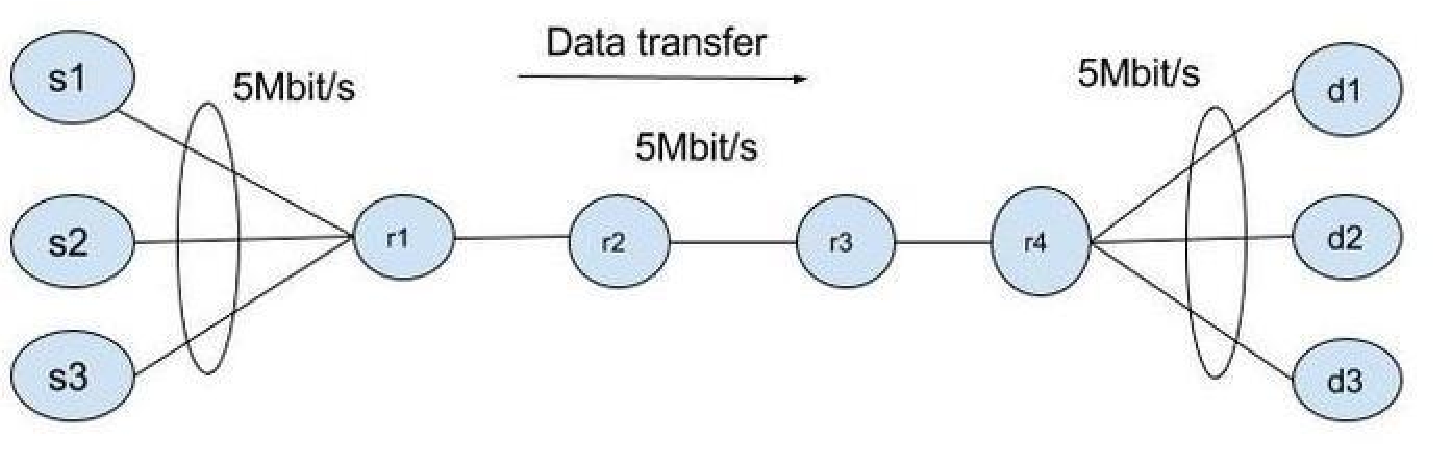
\includegraphics[width=5.5in]{Figures/dumbbell}
\caption{3 Sender-Receiver pair Dumbbell Topology}
\end{center}
\end{figure}
\noindent

\section{Parameters}
The size of payload both in ALFEC--UDP and TCP variants was segmented into 1000 bytes (B). We consider 3 senders transmitting data of length 1MB, 2MB, 3MB to its respective receiver each separately over bandwidth link with a capacity of 5Mbit/s. The rate error model of ns3, that is used to corrupt packets, was applied to all the protocols used for comparison on top of the wired point-to-point link in order to create a loss in the channel. The loss rate considered was in the unit of a packet and it varied from 0, 2, 5 and 10\% of the data length respectively.

For each data length, the \textit{K} value, that is a number of source symbols considered was \textit{K = 1024} and number of source blocks were 1, 2 and 3 for data of length 1MB, 2MB, and 3MB respectively. The time that each sender started to transmit the data was randomized between the range of 0 to 5. As ALFEC--UDP required the redundancy parameter (overhead) to encode the data, we also randomize the overhead between the range of 25\% to 35\% in terms of the total data length for each sender. For each receiver to start the process of decoding, it is required to receive any subset of original length plus 5\% overhead for each block, since \cite{mackay2005fountain} suggests raptor codes can easily be implemented with an overhead of 0.05 in practice. Finally, all our results were averaged over to at least 50 simulation runs. 

\section{Metrics}
Average completion time of data transport using ALFEC--UDP, TCP - New Reno and TCP - HighSpeed protocols; for all 3 sender receiver pairs was calculated at loss rates 0, 2, 5, 10\% respectively. For ALFEC--UDP, we also record the average completion time to complete data transfer for each flow individually.

\section{Results and Discussion}

Figure \ref{r1} displays the result for the 3 sender-receiver pairs in dumbbell topology with each sender transferring 1MB data to the receiver over bandwidth capacity of 5Mbits/s. The X-axis represents the loss percentage applied during the data transport and the
\begin{figure}[htbp] 
\begin{center}
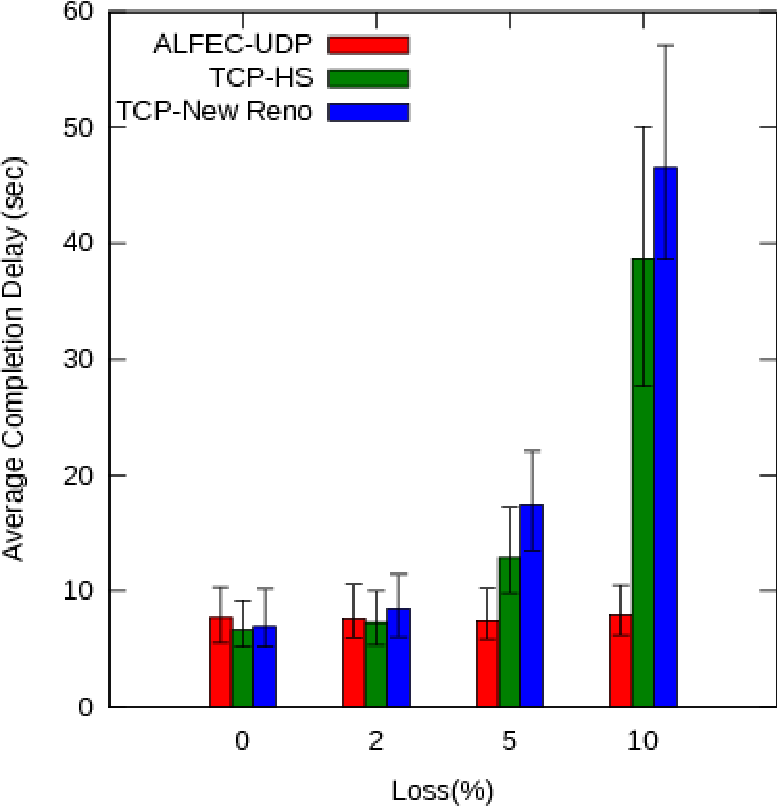
\includegraphics[width=2.5in]{Figures/res1}
\caption{3 sender-receiver pairs each sender transmitting 1MB data over 5Mbits/s capacity link, 0, 2, 5 and 10\% packet loss rate vs Average delay}
\label{r1}
\end{center}
\end{figure}
\noindent
Y-axis represents the average delay taken to complete the simulation. The simulation stopped only after each user received 1MB data and recovered the original data successfully by decoding. During these simulations the packet loss rate was only varied. The bottleneck capacity and size of the data remained constant. In all cases, we used average delay (time taken to complete all 3 users data transfer and recovery) as the performance metric. To evaluate the behavior of ALFEC--UDP, it was compared with two TCP versions, namely TCP New Reno and Highspeed. The figure \ref{r1} clearly indicates that ALFEC--UDP significantly outperforms both TCP versions in terms of average delay even in 10\% lossy environment, showing ALFEC--UDP is less sensitive to the loss.
\begin{figure}[htbp]
\begin{center}
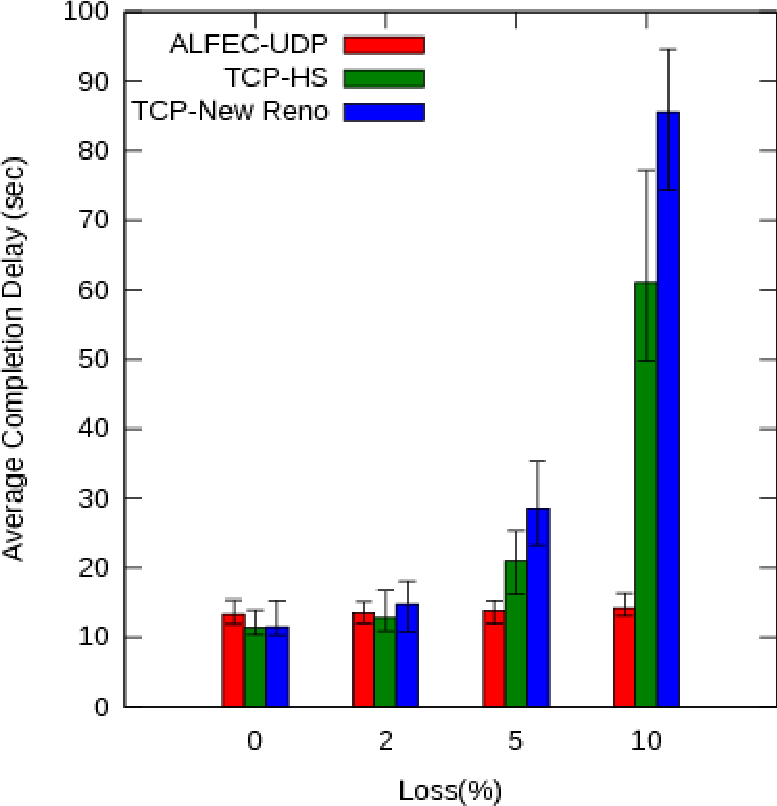
\includegraphics[width=2.5in]{Figures/res2}
\caption{3 sender-receiver pairs each sender transmitting 2MB data over 5Mbits/s capacity link, 0, 2, 5 and 10\% packet loss rate vs Average delay}
\label{r2}
\end{center}
\end{figure}
Error bars represents the minimum and maximum delay that the receivers experienced while completing the whole recovery of data. The minimum and maximum values are ranked based on the 25th and 75th percentile of all the 50 experiments performed.
%\todo[inline]{still very large errorbars! You can lower the percentile.}

The second and third experiment was set with the same setup, but the data length to transfer was increased from 1MB to 2MB and 3MB. Similar metrics as mentioned above were taken into consideration. From figures \ref{r2} and \ref{r3}, it is clearly that ALFEC--UDP does not perform well then both TCP variants for the loss rate of 0 and 2\% due to the fact that it required to receiving the overhead data packets in order to start the process of decoding. But as the loss percent rate is increased, ALFEC--UDP outperforms the TCP variants again showing it to be less sensitive in a lossy environment. ALFEC--UDP on average is approximately 35\% and 25\%  better than TCP variants in terms of average delay in receiving data of length 2MB and 3MB respectively.
\begin{figure}[htbp]
\begin{center}
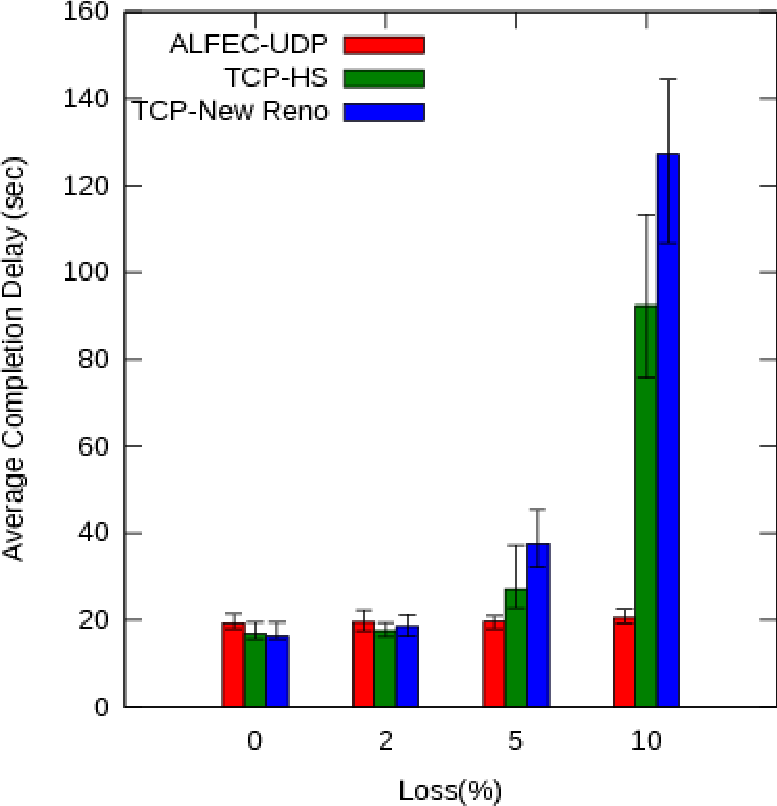
\includegraphics[width=2.5in]{Figures/res3}
\caption{3 sender-receiver pairs each sender transmitting 3MB data over 5Mbits/s capacity link, 0, 2, 5 and 10\% packet loss rate vs Average delay}
\label{r3}
\end{center}
\end{figure}

\begin{figure}[htbp]
\begin{center}
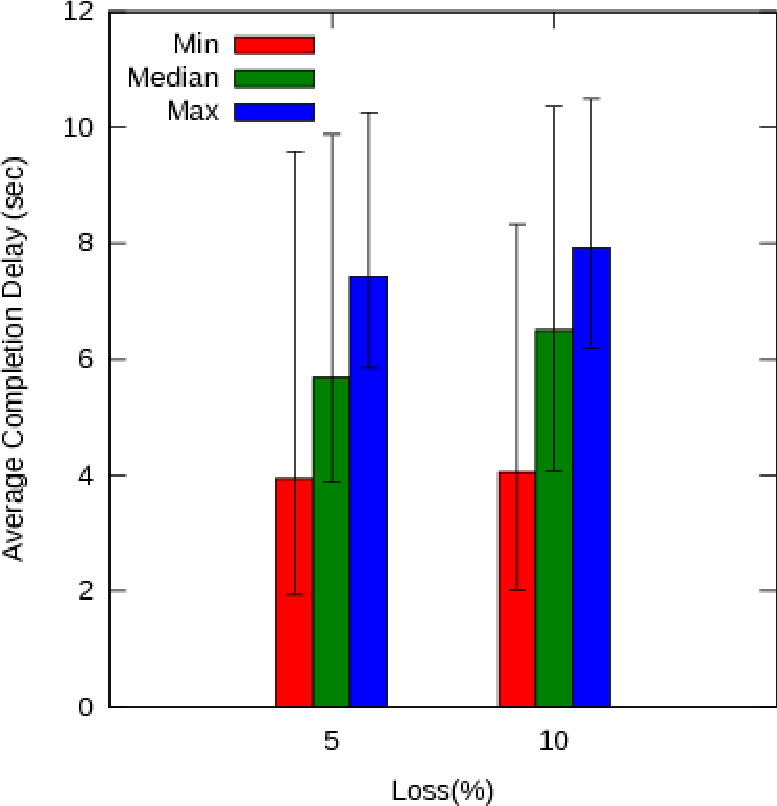
\includegraphics[width=2.5in]{Figures/user1mb}
\caption{3 sender-receiver pairs each transmitting 1MB data over 5Mbits/s, 5\% and 10\% packet loss rate vs each receiver's Average delay}
\label{user1}
\end{center}
\end{figure}

\begin{figure}[htbp]
\begin{center}
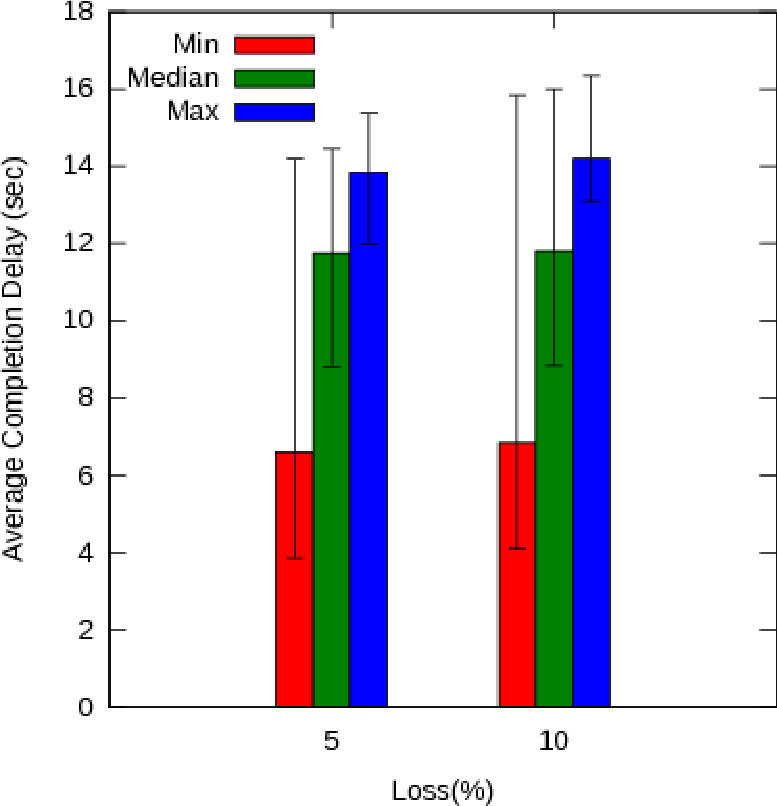
\includegraphics[width=2.5in]{Figures/user2mb}
\caption{3 sender-receiver pairs each transmitting 2MB data over 5Mbits/s, 5\% and 10\% packet loss rate vs each receiver's Average delay}
\label{user2}
\end{center}
\end{figure}

\begin{figure}[htbp]
\begin{center}
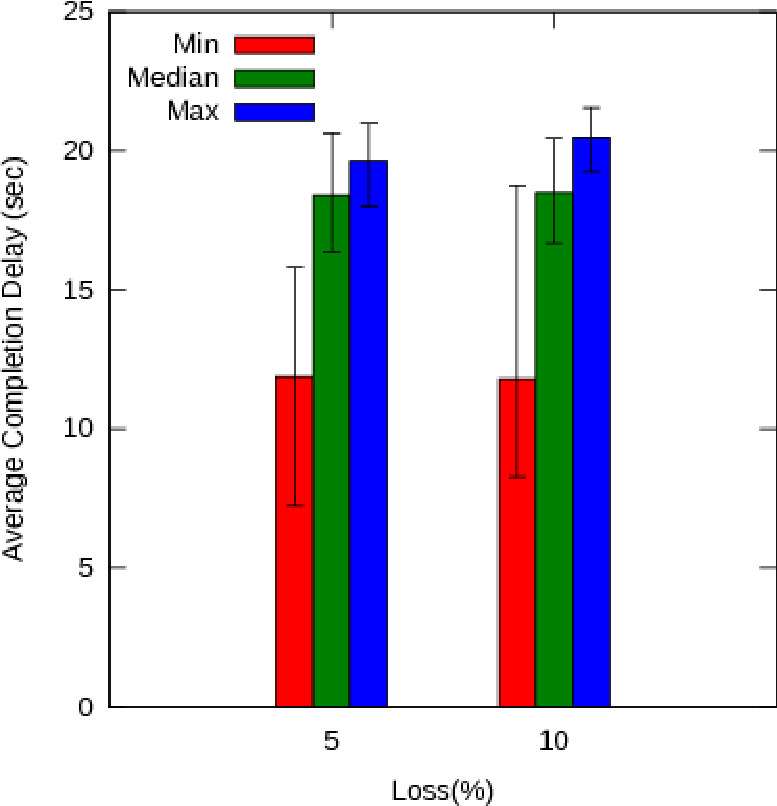
\includegraphics[width=2.5in]{Figures/user3mb}
\caption{3 sender-receiver pairs each transmitting 3MB data over 5Mbits/s, 5\% and 10\% packet loss rate vs each receiver's Average delay}
\label{user3}
\end{center}
\end{figure}


As ALFEC--UDP protocol is developed and implemented using UDP, there is an absence of sequencing and connection oriented data delivery property. There is no guarantee on sequence data delivery and on all the users receiving the total data as there might also be a delay in different routers between the path from the sender to the receiver in packet communication by ALFEC--UDP. Therefore, we record the average completion time of each user in the topology. 

Figures \ref{user1}, \ref{user2} and \ref{user3} shows the average delay each user experience on completely receiving the total data, processing it and decoding successfully. It is clear that no user is starved during the communication. As protocol does not require reordering, the processing time of each packet is also minimized. Any subset of the packet is useful for decoding since each packet has information about the original data.
